%% Per aspera ad astra.
% !TeX spellcheck = pl_PL
%%%%%%%%%%%%%%%%%%%%%%%%%%%%%%%%%%%%%%%%%%%
%                                        %
% Szablon pracy dyplomowej inzynierskiej %
% zgodny  z aktualnymi  przepisami  SZJK %
%                                        %
%%%%%%%%%%%%%%%%%%%%%%%%%%%%%%%%%%%%%%%%%%
%                                        %
%  (c) Krzysztof Simiński, 2018-2023     %
%                                        %
%%%%%%%%%%%%%%%%%%%%%%%%%%%%%%%%%%%%%%%%%%
%                                        %
% Najnowsza wersja szablonów jest        %
% podstępna pod adresem                  %
% github.com/ksiminski/polsl-aei-theses  %
%                                        %
%%%%%%%%%%%%%%%%%%%%%%%%%%%%%%%%%%%%%%%%%%
%
% Projekt LaTeXowy zapewnia odpowiednie formatowanie pracy,
% zgodnie z wymaganiami Systemu zapewniania jakości kształcenia.
% Proszę nie zmieniać ustawień formatowania (np. fontu,
% marginesów, wytłuszczeń, kursywy itd. ).
%
% Projekt można kompilować na kilka sposobów.
%
% 1. kompilacja pdfLaTeX
%
% pdflatex main
% bibtex   main
% pdflatex main
% pdflatex main
%
% 2. kompilacja XeLaTeX
%
% Kompilatacja przy użyciu XeLaTeXa różni się tym, że na stronie
% tytułowej używany jest font Calibri. Wymaga to jego uprzedniego
% zainstalowania.
%
% xelatex main
% bibtex  main
% xelatex main
% xelatex main
%
%%%%%%%%%%%%%%%%%%%%%%%%%%%%%%%%%%%%%%%%%%%%%%%%%%%%%
% W przypadku pytań, uwag, proszę pisać na adres:   %
%      krzysztof.siminski(małpa)polsl.pl            %
%%%%%%%%%%%%%%%%%%%%%%%%%%%%%%%%%%%%%%%%%%%%%%%%%%%%%
%
% Chcemy ulepszać szablony LaTeXowe prac dyplomowych.
% Wypełniając ankietę spod poniższego adresu pomogą
% Państwo nam to zrobić. Ankieta jest całkowicie
% anonimowa. Dziękujemy!

% https://docs.google.com/forms/d/e/1FAIpQLScyllVxNKzKFHfILDfdbwC-jvT8YL0RSTFs-s27UGw9CKn-fQ/viewform?usp=sf_link
%
%%%%%%%%%%%%%%%%%%%%%%%%%%%%%%%%%%%%%%%%%%%%%%%%%%%%%%%%%%%%%%%%%%%%%%%%%

% Autor pracy inżynierskiej na bazie szablonu,
% oraz wszelkich poprawek:
% Daniel Chydziński

%%%%%%%%%%%%%%%%%%%%%%%%%%%%%%%%%%%%%%%%%%%%%%%
%                                             %
% PERSONALIZACJA PRACY – DANE PRACY           %
%                                             %
%%%%%%%%%%%%%%%%%%%%%%%%%%%%%%%%%%%%%%%%%%%%%%%

% Proszę wpisać swoje dane w poniższych definicjach.

% TODO
% dane autora
\newcommand{\FirstNameAuthor}{Daniel}
\newcommand{\SurnameAuthor}{Chydziński}
\newcommand{\IdAuthor}{296781}

% drugi autor:
%\newcommand{\FirstNameCoauthor}{Imię}   % Jeżeli jest drugi autor, to tutaj należy podać imię.
%\newcommand{\SurnameCoauthor}{Nazwisko} % Jeżeli jest drugi autor, to tutaj należy podać nazwisko.
%\newcommand{\IdCoauthor}{$\langle$wpisać właściwy$\rangle$}  % numer albumu drugiego autora (bez $\langle$ i $\rangle$)
% Gdy nie ma drugiego autora, należy zostawić poniższe definicje puste, jak poniżej. Gdy jest drugi autor, należy zakomentować te linie.
\newcommand{\FirstNameCoauthor}{} % Jeżeli praca ma tylko jednego autora, to dane drugiego autora zostają puste.
\newcommand{\SurnameCoauthor}{}   % Jeżeli praca ma tylko jednego autora, to dane drugiego autora zostają puste.
\newcommand{\IdCoauthor}{}  % Jeżeli praca ma tylko jednego autora, to dane drugiego autora zostają puste.
%%%%%%%%%%

\newcommand{\Supervisor}{dr Aleksander Staszulonek}     % dane promotora (bez $\langle$ i $\rangle$)
\newcommand{\Title}{Analiza błędów pomiaru położenia platformy mobilnej}           % tytuł pracy po polsku
\newcommand{\TitleAlt}{Mobile platform position errors analysis}                     % thesis title in English
\newcommand{\Program}{Automatyka i Robotyka}            % kierunek studiów  (bez $\langle$ i $\rangle$)
\newcommand{\Specialisation}{Automatyka Procesowa}     % specjalność  (bez $\langle$ i $\rangle$)
\newcommand{\Departament}{Automatyki i Robotyki}        % katedra promotora  (bez $\langle$ i $\rangle$)

% Jeżeli został wyznaczony promotor pomocniczy lub opiekun, proszę go/ją wpisać ...
\newcommand{\Consultant}{$\langle$stopień naukowy imię i nazwisko$\rangle$} % dane promotora pomocniczego, opiekuna (bez $\langle$ i $\rangle$)
% ... w przeciwnym razie proszę zostawić puste miejsce jak poniżej:
%\newcommand{\Consultant}{} % brak promotowa pomocniczego / opiekuna

% koniec fragmentu do modyfikacji
%%%%%%%%%%%%%%%%%%%%%%%%%%%%%%%%%%%%%%%%%%

%%%%%%%%%%%%%%%%%%%%%%%%%%%%%%%%%%%%%%%%%%%%%%%
%                                             %
% KONIEC PERSONALIZACJI PRACY                 %
%                                             %
%%%%%%%%%%%%%%%%%%%%%%%%%%%%%%%%%%%%%%%%%%%%%%%

%%%%%%%%%%%%%%%%%%%%%%%%%%%%%%%%%%%%%%%%%%%%%%%
%                                             %
% PROSZĘ NIE MODYFIKOWAĆ PONIŻSZYCH USTAWIEŃ! %
%                                             %
%%%%%%%%%%%%%%%%%%%%%%%%%%%%%%%%%%%%%%%%%%%%%%%

\documentclass[a4paper,twoside,12pt]{book}
\usepackage[utf8]{inputenc}                                      
\usepackage[T1]{fontenc}  
\usepackage{amsmath,amsfonts,amssymb,amsthm}
\usepackage[british,polish]{babel} 
\usepackage{indentfirst}
\usepackage{xurl}
\usepackage{xstring}
\usepackage{ifthen}



\usepackage{ifxetex}

\ifxetex
	\usepackage{fontspec}
	\defaultfontfeatures{Mapping=tex—text} % to support TeX conventions like ``——-''
	\usepackage{xunicode} % Unicode support for LaTeX character names (accents, European chars, etc)
	\usepackage{xltxtra} % Extra customizations for XeLaTeX
\else
	\usepackage{lmodern}
\fi



\usepackage[margin=2.5cm]{geometry}
\usepackage{graphicx} 
\usepackage{hyperref}
\usepackage{booktabs}
\usepackage{tikz}
\usepackage{pgfplots}
\usepackage{mathtools}
\usepackage{geometry}
\usepackage{subfig}   % subfigures
\usepackage[page]{appendix} % toc,
\renewcommand{\appendixtocname}{Dodatki}
\renewcommand{\appendixpagename}{Dodatki}
\renewcommand{\appendixname}{Dodatek}

\usepackage{csquotes}
\usepackage[natbib=true,backend=bibtex,maxbibnames=99]{biblatex}  % kompilacja bibliografii BibTeXem
%\usepackage[natbib=true,backend=biber,maxbibnames=99]{biblatex}  % kompilacja bibliografii Biberem
\bibliography{biblio}

\usepackage{ifmtarg}   % empty commands  

\usepackage{setspace}
\onehalfspacing


\frenchspacing

%%%%%%%%%%%%%%%%%%%%%%%%%%%%%%%%%%
% środowiska dla definicji, twierdzenia, przykładu
\usepackage{amsthm}

\newtheorem{Definition}{Definicja}
\newtheorem{Example}{Przykład}
\newtheorem{Theorem}{Twierdzenie}
%%%%%%%%%%%%%%%%%%%%%%%%%%%%%%%%%%

%%%% TODO LIST GENERATOR %%%%%%%%%

\usepackage{color}
\definecolor{brickred}      {cmyk}{0   , 0.89, 0.94, 0.28}

\makeatletter \newcommand \kslistofremarks{\section*{Uwagi} \@starttoc{rks}}
  \newcommand\l@uwagas[2]
    {\par\noindent \textbf{#2:} %\parbox{10cm}
{#1}\par} \makeatother


\newcommand{\ksremark}[1]{%
{%\marginpar{\textdbend}
{\color{brickred}{[#1]}}}%
\addcontentsline{rks}{uwagas}{\protect{#1}}%
}

\newcommand{\comma}{\ksremark{przecinek}}
\newcommand{\nocomma}{\ksremark{bez przecinka}}
\newcommand{\styl}{\ksremark{styl}}
\newcommand{\ortografia}{\ksremark{ortografia}}
\newcommand{\fleksja}{\ksremark{fleksja}}
\newcommand{\pauza}{\ksremark{pauza `--', nie dywiz `-'}}
\newcommand{\kolokwializm}{\ksremark{kolokwializm}}
\newcommand{\cudzyslowy}{\ksremark{,,polskie cudzysłowy''}}

%%%%%%%%%%%%%% END OF TODO LIST GENERATOR %%%%%%%%%%%

\newcommand{\printCoauthor}{%		
    \StrLen{\FirstNameCoauthor}[\FNCoALen]
    \ifthenelse{\FNCoALen > 0}%
    {%
		{\large\bfseries\Coauthor\par}
	
		{\normalsize\bfseries \LeftId: \IdCoauthor\par}
    }%
    {}
} 

%%%%%%%%%%%%%%%%%%%%%
\newcommand{\autor}{%		
    \StrLen{\FirstNameCoauthor}[\FNCoALenXX]
    \ifthenelse{\FNCoALenXX > 0}%
    {\FirstNameAuthor\ \SurnameAuthor, \FirstNameCoauthor\ \SurnameCoauthor}%
	{\FirstNameAuthor\ \SurnameAuthor}%
}
%%%%%%%%%%%%%%%%%%%%%

\StrLen{\FirstNameCoauthor}[\FNCoALen]
\ifthenelse{\FNCoALen > 0}%
{%
\author{\FirstNameAuthor\ \SurnameAuthor, \FirstNameCoauthor\ \SurnameCoauthor}
}%
{%
\author{\FirstNameAuthor\ \SurnameAuthor}
}%

%%%%%%%%%%%% ZYWA PAGINA %%%%%%%%%%%%%%%
% brak kapitalizacji zywej paginy
\usepackage{fancyhdr}
\pagestyle{fancy}
\fancyhf{}
\fancyhead[LO]{\nouppercase{\it\rightmark}}
\fancyhead[RE]{\nouppercase{\it\leftmark}}
\fancyhead[LE,RO]{\it\thepage}


\fancypagestyle{tylkoNumeryStron}{%
   \fancyhf{} 
   \fancyhead[LE,RO]{\it\thepage}
}

\fancypagestyle{bezNumeracji}{%
   \fancyhf{} 
   \fancyhead[LE,RO]{}
}


\fancypagestyle{NumeryStronNazwyRozdzialow}{%
   \fancyhf{} 
   \fancyhead[LE]{\nouppercase{\autor}}
   \fancyhead[RO]{\nouppercase{\leftmark}} 
   \fancyfoot[CE, CO]{\thepage}
}


%%%%%%%%%%%%% OBCE WTRETY  
\newcommand{\obcy}[1]{\emph{#1}}
\newcommand{\english}[1]{{\selectlanguage{british}\obcy{#1}}}
%%%%%%%%%%%%%%%%%%%%%%%%%%%%%

% polskie oznaczenia funkcji matematycznych
\renewcommand{\tan}{\operatorname {tg}}
\renewcommand{\log}{\operatorname {lg}}

% jeszcze jakies drobiazgi

\newcounter{stronyPozaNumeracja}

%%%%%%%%%%%%%%%%%%%%%%%%%%% 
\newcommand{\printOpiekun}[1]{%		

    \StrLen{\Consultant}[\mystringlen]
    \ifthenelse{\mystringlen > 0}%
    {%
       {\large{\bfseries OPIEKUN, PROMOTOR POMOCNICZY}\par}
       
       {\large{\bfseries \Consultant}\par}
    }%
    {}
} 
%
%%%%%%%%%%%%%%%%%%%%%%%%%%%%%%%%%%%%%%%%%%%%%%
 
% Proszę nie modyfikować poniższych definicji!
\newcommand{\Author}{\FirstNameAuthor\ \MakeUppercase{\SurnameAuthor}} 
\newcommand{\Coauthor}{\FirstNameCoauthor\ \MakeUppercase{\SurnameCoauthor}}
\newcommand{\Type}{PROJEKT INŻYNIERSKI}
\newcommand{\Faculty}{Wydział Automatyki, Elektroniki i Informatyki} 
\newcommand{\Polsl}{Politechnika Śląska}
\newcommand{\Logo}{politechnika_sl_logo_bw_pion_pl.pdf}
\newcommand{\LeftId}{Nr albumu}
\newcommand{\LeftProgram}{Kierunek}
\newcommand{\LeftSpecialisation}{Specjalność}
\newcommand{\LeftSUPERVISOR}{PROWADZĄCY PRACĘ}
\newcommand{\LeftDEPARTMENT}{KATEDRA}
%%%%%%%%%%%%%%%%%%%%%%%%%%%%%%%%%%%%%%%%%%%%%%

%%%%%%%%%%%%%%%%%%%%%%%%%%%%%%%%%%%%%%%%%%%%%%%
%                                             %
% KONIEC USTAWIEŃ                             %
%                                             %
%%%%%%%%%%%%%%%%%%%%%%%%%%%%%%%%%%%%%%%%%%%%%%%

%%%%%%%%%%%%%%%%%%%%%%%%%%%%%%%%%%%%%%%%%%%%%%%
%                                             %
% MOJE PAKIETY, USTAWIENIA ITD                %
%                                             %
%%%%%%%%%%%%%%%%%%%%%%%%%%%%%%%%%%%%%%%%%%%%%%%

% Tutaj proszę umieszczać swoje pakiety, makra, ustawienia itd.


 
%%%%%%%%%%%%%%%%%%%%%%%%%%%%%%%%%%%%%%%%%%%%%%%%%%%%%%%%%%%%%%%%%%%%%
% listingi i fragmentu kodu źródłowego 
% pakiet: listings lub minted
% % % % % % % % % % % % % % % % % % % % % % % % % % % % % % % % % % % 

% biblioteka listings
\usepackage{listings}
\lstset{%
morekeywords={string,exception,std,vector},% słowa kluczowe rozpoznawane przez pakiet listings
language=C++,% C, Matlab, Python, SQL, TeX, XML, bash, ... – vide https://www.ctan.org/pkg/listings
commentstyle=\textit,%
identifierstyle=\textsf,%
keywordstyle=\sffamily\bfseries, %\texttt, %
%captionpos=b,%
tabsize=3,%
frame=lines,%
numbers=left,%
numberstyle=\tiny,%
numbersep=5pt,%
breaklines=true,%
escapeinside={@*}{*@},%
}

\usepackage{enumerate}

% % % % % % % % % % % % % % % % % % % % % % % % % % % % % % % % % % % 
% pakiet minted
%\usepackage{minted}

% pakiet wymaga specjalnego kompilowania:
% pdflatex -shell-escape main.tex
% xelatex  -shell-escape main.tex

%\usepackage[chapter]{minted} % [section]
%%\usemintedstyle{bw}   % czarno-białe kody 
%
%\setminted % https://ctan.org/pkg/minted
%{
%%fontsize=\normalsize,%\footnotesize,
%%captionpos=b,%
%tabsize=3,%
%frame=lines,%
%framesep=2mm,
%numbers=left,%
%numbersep=5pt,%
%breaklines=true,%
%escapeinside=@@,%
%}

%%%%%%%%%%%%%%%%%%%%%%%%%%%%%%%%%%%%%%%%%%%%%%%%%%%%%%%%%%%%%%%%%%%%%

%%%%%%%%%%%%%%%%%%%%%%%%%%%%%%%%%%%%%%%%%%%%%%%
%                                             %
% KONIEC MOICH USTAWIEŃ                       %
%                                             %
%%%%%%%%%%%%%%%%%%%%%%%%%%%%%%%%%%%%%%%%%%%%%%%

\begin{document}
%\kslistofremarks

\frontmatter

%%%%%%%%%%%%%%%%%%%%%%%%%%%%%%%%%%%%%%%%%%%%%%%
%                                             %
% PROSZĘ NIE MODYFIKOWAĆ STRONY TYTUŁOWEJ!    %
%                                             %
%%%%%%%%%%%%%%%%%%%%%%%%%%%%%%%%%%%%%%%%%%%%%%%

\pagestyle{empty}
{
	\newgeometry{top=1.5cm,%
	             bottom=2.5cm,%
	             left=3cm,
	             right=2.5cm}
 
	\ifxetex 
	  \begingroup
	  \setsansfont{Calibri}
	   
	\fi 
	 \sffamily
	\begin{center}
	\includegraphics[width=100mm]{\Logo}
	 
	
	{\Large\bfseries\Type\par}
	
	\vfill  \vfill  
			 
	{\large\Title\par}
	
	\vfill  
		
	{\large\bfseries\Author\par}
	
	{\normalsize\bfseries \LeftId: \IdAuthor}

	\printCoauthor
	
	\vfill  		
 
	{\large{\bfseries \LeftProgram:} \Program\par} 
	
	{\large{\bfseries \LeftSpecialisation:} \Specialisation\par} 
	 		
	\vfill  \vfill 	\vfill 	\vfill 	\vfill 	\vfill 	\vfill  
	 
	{\large{\bfseries \LeftSUPERVISOR}\par}
	
	{\large{\bfseries \Supervisor}\par}
				
	{\large{\bfseries \LeftDEPARTMENT\ \Departament} \par}
		
	{\large{\bfseries \Faculty}\par}
		
	\vfill  \vfill  

    
	\vfill  \vfill  
		
    {\large\bfseries  Gliwice \the\year}

   \end{center}	
       \ifxetex 
       	  \endgroup
       \fi
	\restoregeometry
}
  
%%%%%%%%%%%%%%%%%%%%%%%%%%%%%%%%%%%%%%%%%%%%%%%
%                                             %
% KONIEC STRONY TYTUŁOWEJ                     %
%                                             %
%%%%%%%%%%%%%%%%%%%%%%%%%%%%%%%%%%%%%%%%%%%%%%%  

\cleardoublepage

\rmfamily\normalfont
\pagestyle{empty}

%%% tu można pisać

\subsubsection*{Tytuł pracy} 
\Title

\subsubsection*{Streszczenie}  
Projekt, wykonanie i testy platformy mobilnej opartej na mikroprocesorze, silnikach prądu stałego z enkoderami i regulatorach PID.

\subsubsection*{Słowa kluczowe} 
Silnik, druk 3D, regulator PID, mikroprocesor

\subsubsection*{Thesis title} 
\begin{otherlanguage}{british}
\TitleAlt
\end{otherlanguage}

\subsubsection*{Abstract} 
\begin{otherlanguage}{british}
Design, development and testing of a mobile platform based on a microprocessor, direct current motors with encoders and PID controllers.
\end{otherlanguage}
\subsubsection*{Key words}  
\begin{otherlanguage}{british}
Motor, 3D printing, PID controller, microprocessor
\end{otherlanguage}

%%%%%%%%%%%%%%%%%% SPIS TRESCI %%%%%%%%%%%%%%%%%%%%%%
% Add \thispagestyle{empty} to the toc file (main.toc), because \pagestyle{empty} doesn't work if the TOC has multiple pages
\addtocontents{toc}{\protect\thispagestyle{empty}}
\tableofcontents

%%%%%%%%%%%%%%%%%%%%%%%%%%%%%%%%%%%%%%%%%%%%%%%%%%%%%
\setcounter{stronyPozaNumeracja}{\value{page}}
\mainmatter
\pagestyle{empty}

\cleardoublepage

\pagestyle{NumeryStronNazwyRozdzialow}

%%%%%%%%%%%%%% wlasciwa tresc pracy %%%%%%%%%%%%%%%%%

%%%%%%%%%%%%%% rozdział 1 - Wstęp %%%%%%%%%%%%%%%%%
\chapter{Wstęp}
\label{ch:wstep}

Robotyka to obszar badawczy i~techniczny poświęcony teorii, konstrukcji oraz praktycznym zastosowaniom robotów. Elementami wykonawczymi układów zrobotyzowanych są najczęściej silniki lub siłowniki, te drugie nierzadko napędzane wewnętrznie silnikami. Rodzajem maszyny zamieniającej jeden rodzaj energii --- w~robotyce najczęściej elektryczną --- na energię mechaniczną, czego celem jest wprawienie w~ruch elementów ruchomych.

W przypadku prostych układów (Definicja~\ref{def:uklad}), takich jak podajnik taśmowy napędzany pojedynczym silnikiem, dokładność (Definicja~\ref{def:dokladnosc}) sterowania nie ma wysokiego priorytetu. Najważniejsze jest, by element znajdujący się na taśmie przejechał z~punktu A~do punktu B~z~pewną prędkością, a~jego położeniem zajmą się inne czujniki. Jednak gdy silnik napędza ramię robota, pojazd lub drona, ważne jest, by utrzymywał stałą prędkość i/lub wykonywał określoną ilość obrotów.

\begin{Definition}[Układ sterowania]\label{def:uklad}
   Układ służący do kontroli pożądanego urządzenia przy pomocy wybranego zasobu narzędzi, w~tym zamkniętej pętli z~ujemnym sprzężeniem zwrotnym (Definicja~\ref{def:petla}).
\end{Definition}

\begin{Definition}[Pętla]\label{def:petla}
    Typ struktury układu umożliwiający mu reakcję na informację zwrotną o~jego stanie (sprzężenie zwrotne) pochodzącą z czujników.
\end{Definition}

\begin{Definition}[Dokładność]\label{def:dokladnosc}
    Stopień zgodności pomiędzy rzeczywistymi wartościami a~wartościami określonymi lub mierzonymi.
\end{Definition}

Z tego powodu, jednym z~wyzwań, z~jakimi mierzyli się pionierzy automatycy-robotycy jest dokładne sterowanie tworzonymi przez siebie układami. Jest to kwestia o~tyle istotna, że gdy odpowiedź układu odbiega --- nawet w niewielkim stopniu --- od wartości zadanej, staje się on znacząco trudniejszy w~użytkowaniu (sterowaniu), a w skrajnych przypadkach bezużyteczny. W~przypadku ramienia robota, brak dokładności sterowania doprowadzi układ do osiągnięcia innej lokalizacji niż pożądana. W~przypadku drona, prawdopodobnie całkowicie uniemożliwi lot z~powodu nierówności sił nośnych. Zaś w~przypadku pojazdów autonomicznych, przejechanie odległości innej niż zadana przez operatora. Jako rozwiązanie tego problemu, powstał poddział robotyki zwany odometrią (Definicja~\ref{def:odometria}). 

\begin{Definition}[Odometria]\label{def:odometria}
    Dział nauk technicznych na pograniczu robotyki i~miernictwa, zajmujący się użyciem różnego rodzaju czujników w~celu oszacowania położenia ruchomego układu względem pozycji startowej w przestrzeni fizycznej.
\end{Definition}

Współcześni automatycy-robotycy będący na początku swojej ścieżki edukacji/kariery, lub zajmujący się robotyką jedynie hobbystycznie, również mierzą się prędzej czy później z~problemem dokładności sterowania układu. W~obecnych czasach istnieje wiele sposobów rozwiązania go.

Celem niniejszej pracy inżynierskiej jest zaprojektowanie i~wykonanie fizycznego modelu platformy mobilnej (zwanej dalej pojazdem) oraz aplikacji do jej kontroli. Następnie zastosowanie i~przetestowanie eksperymentalne wybranej metody zwiększenia dokładności układu z~użyciem ujemnego sprzężenia zwrotnego. Na końcu otrzymane wyniki zostaną przeanalizowane pod kątem użyteczności i skuteczności wybranej metody w warunkach rzeczywistych.

Praca podzielona została na następujące rozdziały\cite{bib:wymaganiapracy}:
\begin{enumerate}
    \item Wstęp --- wprowadzenie do tematu, krótkie omówienie istoty problemu, zakres pracy, opis rozdziałów.
    \item Analiza tematu --- omówienie tematu w kontekście aktualnego stanu wiedzy o poruszanym problemie (ang. \english{state of art}), oraz szczegółowe jego sformułowanie.
    \item Założenia i narzędzia --- opis wymagań postawionych przy tworzeniu projektu wraz z uzasadnieniem wyboru, a także lista użytych narzędzi.
    \item Projekt i wykonanie --- szczegółowe omówienie sposobu wykonania modelu pojazdu, układu elektronicznego, aplikacji, kodu mikroprocesora i narzędzi pobocznych. Każdemu elementowi odpowiada podrozdział.
    \item Weryfikacja i walidacja --- zastosowane metody badawcze i wykonane eksperymenty, oraz napotkane i usunięte błędy.
    \item Podsumowanie i wnioski --- skomentowanie uzyskanych wyników pod kątem osiągnięcia założonych celów, analiza i dalsze kroki.
\end{enumerate}

%%%%%%%%%%%%%% rozdział 2 - Analiza %%%%%%%%%%%%%%%%%
\chapter{Analiza tematu}
\section{Detekcja położenia wału silnika}
\label{ch:analizaenkodery}

Problem synchronizowania silników elektrycznych znany jest w~dziedzinie automatyki od dziesiątek lat. Początki badania silników sięgają XIX wieku, kiedy to Michael Faraday oraz inni naukowcy eksperymentowali ze wykorzystaniem elektromagnetyzmu\cite{bib:pierwszesilniki}. Pierwsze silniki elektryczne były prymitywne i~nie miały zaawansowanych metod sterowania. Wczesne próby pozycjonowania opierały się głównie na prostych mechanizmach, takich jak przekładnie i~sprzęgła.

W miarę postępu technologicznego, szczególnie w~XX wieku, rozwijano bardziej zaawansowane metody pozycjonowania. Pojawiły się pierwsze systemy sterowania, wykorzystujące technologię zwrotną informacji, mającą na celu monitorowanie i~regulację położenia wałów silników. Jednak precyzja tych rozwiązań była ograniczona, a~dokładność pozycjonowania nie zawsze spełniała wymagania coraz bardziej zaawansowanych zastosowań.

Dopiero wprowadzenie enkoderów (Definicja~\ref{def:enkoder}) elektronicznych w~latach 60.~XX~wieku\cite{bib:pierwszeenkodery} stało się przełomem.

\begin{Definition}[Enkoder obrotowy]\label{def:enkoder}
    Urządzenie, generujące sygnały elektryczne odpowiadające ruchowi obrotowemu wału silnika celem określenia jego pozycji. 
\end{Definition}

Początkowo enkodery były oparte na szczotkach stykających się z dyskiem zawierającym serię odpowiednio zakodowanych pierścieni koncentrycznych (Rysunek~\ref{fig:encoderDiscAbsolute}), wypełnionych otworami o odpowiedniej długości\cite{bib:rodzajeenkoderow}. Są one tanie w~produkcji, jednak mają swoje ograniczenia związane ze zużyciem mechanicznym elementów stykowych, niską maksymalną dozwoloną prędkością silnika i~wymaganiami konserwacji. Ten typ enkoderów spotykany jest do dziś, na przykład w multimetrach cyfrowych.

Rozwój technologii przyniósł enkodery optyczne, wykorzystujące diody LED i~fotodetektory. Później pojawiły się enkodery magnetyczne. To właśnie one --- enkodery optyczne i~magnetyczne --- są do dnia dzisiejszego najczęściej spotykane i~oferują najwyższą dokładność sterowania przy niskich kosztach i~niewielkim stopniu skomplikowania. To właśnie na nich skupiono się w~dalszej części pracy.

Enkodery można podzielić ze względu na\cite{bib:rodzajeenkoderow}:
\begin{itemize}
    \item Metodę używaną do odczytania pozycji: kontaktowe i~bezkontaktowe.
    \item Rodzaj sygnału wyjściowego: pozycja absolutna lub szereg inkrementujących/dekrementujących wartości.
    \item Zjawisko fizyczne wykorzystane do przesłania sygnału pozycyjnego: przewodzenie elektryczne, magnetyzm, zjawiska optyczne lub pojemnościowe.
\end{itemize}

Najważniejszy jest podział ze względu na rodzaj sygnału wyjściowego. Mimo, że zarówno enkodery absolutne jak i~inkrementalne posiadają dyski kodujące, różnią się one działaniem. Enkodery absolutne jako sygnał wyjściowy podają precyzyjną pozycję wału silnika, najczęściej zakodowaną w~słowie bitowym. Przykładowy wygląd dysku kodującego widoczny jest na Rysunku~\ref{fig:encoderDiscAbsolute}. Istotną cechą tego rodzaju enkoderów jest możliwość określenia pozycji nawet po utracie zasilania.

\begin{center}
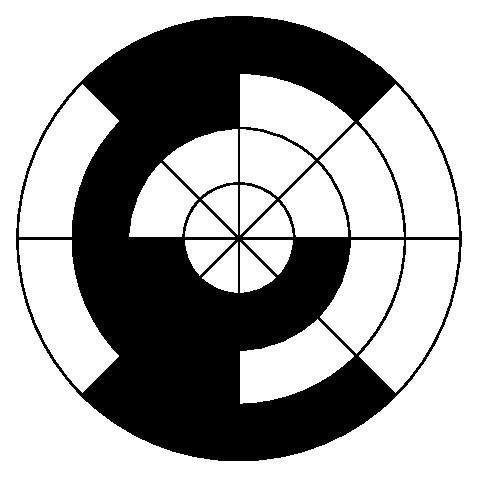
\includegraphics[scale=1]{images/encoderDiscAbsolute.eps}
\captionof{figure}{Poglądowy schemat dysku enkodera absolutnego z 3-bitowym kodem Graya\cite{bib:tarczaenkoderaabsolutnego}}
\label{fig:encoderDiscAbsolute}
\end{center}

Enkodery inkrementalne u~podstaw działają~w ten sam sposób, tzn. opierają się na dyskach kodujących, z~tą różnicą, że nie są w~stanie podać dokładnej wartości położenia. Zamiast tego, podają na wyjściu odpowiedni impuls przy obrocie w~danym kierunku. Następnie w~oprogramowaniu impulsy te są zliczane w celu oszacowania aktualnej pozycji względem pozycji startowej. Ze względu na wyzerowanie liczby impulsów przy utracie zasilania, ten typ enkodera nie jest w~stanie podać dokładnej pozycji w~przypadku utraty zasilania.

Istotny jest również podział enkoderów ze względu na wykorzystywane zjawisko fizyczne. Dwa główne typy to enkodery optyczne oraz magnetyczne. Oba rodzaje występują zarówno w~wariancie pojedynczym (Rysunek~\ref{fig:encoderDiscIncrementalSingle}) jak i~podwójnym (Rysunek~\ref{fig:encoderDiscIncrementalDual}). W~przypadku enkoderów optycznych, kolorowi białemu odpowiada szczelina, zaś kolorowi czarnemu blokada. W~przypadku enkoderów magnetycznych, kolorom odopowiadają bieguny~S~i~N.

\begin{figure}
    \centering
    \subfloat[Enkoder pojedynczy]{
      
\includegraphics[width=5cm]{images/encoderDiscIncrementalSingle.eps}
      \label{fig:encoderDiscIncrementalSingle}
    }\qquad
    \subfloat[Enkoder podwójny (kwadratowy)]{
      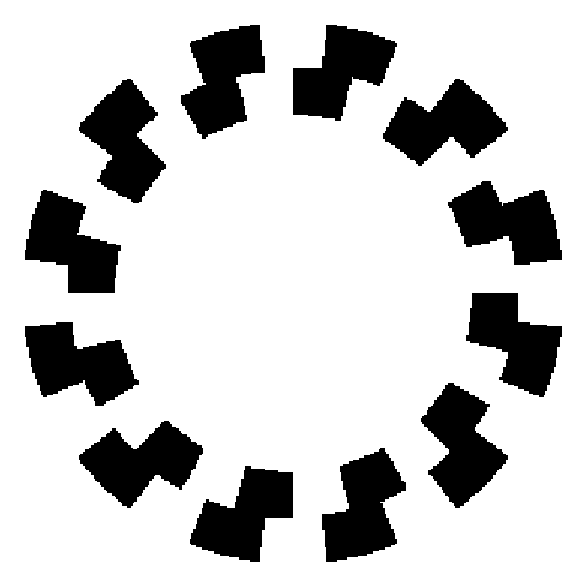
\includegraphics[width=5cm]{images/encoderDiscIncrementalDual.eps}
      \label{fig:encoderDiscIncrementalDual}
    }
    \caption{Poglądowe schematy dysku enkodera inkrementalnego \cite{bib:tarczeenkoderowinkrementalnych}}
\end{figure}

Jako że w~projekcie wykorzystane zostały enkodery magnetyczne, zasada ich działania została opisana, zaś enkodery optyczne pominięto. W enkoderze magnetycznym umieszcza się magnesy na obracającej się lub przemieszczającej się części obiektu~---~czyli dysku~---~a~czujniki magnetyczne~---~najczęściej czujniki Halla (Definicja~\ref{def:czujnikhalla})~---~znajdujące się na stałej części enkodera rejestrują zmiany pola magnetycznego (Rysunek~\ref{fig:obrazekenkoderamagnetycznego}). 

\begin{center}
  \includegraphics[scale=0.08]{images/magneticEncoder.png}
  \captionof{figure}{Zobrazowanie zasady działania enkodera magnetycznego dla tarczy z jednym rzędem\cite{bib:obrazekenkoderamagnetycznego}}
  \label{fig:obrazekenkoderamagnetycznego}
\end{center}

\begin{Definition}[Czujnik Halla]\label{def:czujnikhalla}
  Czujnik pola magnetycznego i~prądu, wykorzystujący zjawisko Halla.
\end{Definition}

Te zmiany są następnie przetwarzane na sygnały elektryczne, które można interpretować jako informacje o~kącie obrotu lub przemieszczeniu. Enkodery magnetyczne charakteryzują się wysoką dokładnością pomiaru, odpornością na wibracje i~brakiem kontaktu mechanicznego, dzięki czemu są odporne na zabrudzenia i~czynniki zewnętrzne takie jak kurz. Nie ma więc potrzeby osadzania ich w~zamkniętej przestrzeni, jak to ma miejsce z~czujnikami optycznymi.

\section{Regulacja sygnału sterującego}
\label{ch:regulatory}
Oprócz urządzenia (czujnika) dostarczającego sygnał informujący o fizycznym położeniu lub przemieszczeniu wału silnika, konieczne jest również zastosowanie metody wyznaczenia sygnału sterującego $u$. 

Trudno jest określić datę powstania pierwszych regulatorów. Pierwotnie nie były one tworzone z~myślą o~wyznaczaniu sygnału sterującego, lecz zwyczajnie jako część urządzeń. Przykładem jednego z~pierwszych regulatorów może być maszyna Ktesibiosa ---~wynaleziona w~III wieku~p.n.e.\cite{bib:regulatorktesibiusa} ---~w której rolę regulatora pełnił pływak dławiący wypływającą ze źródła wodę (Rysunek~\ref{fig:ktesibius}). Jest to prawdopodobnie pierwszy na świecie przykład regulatora proporcjonalnego.

\begin{center}
  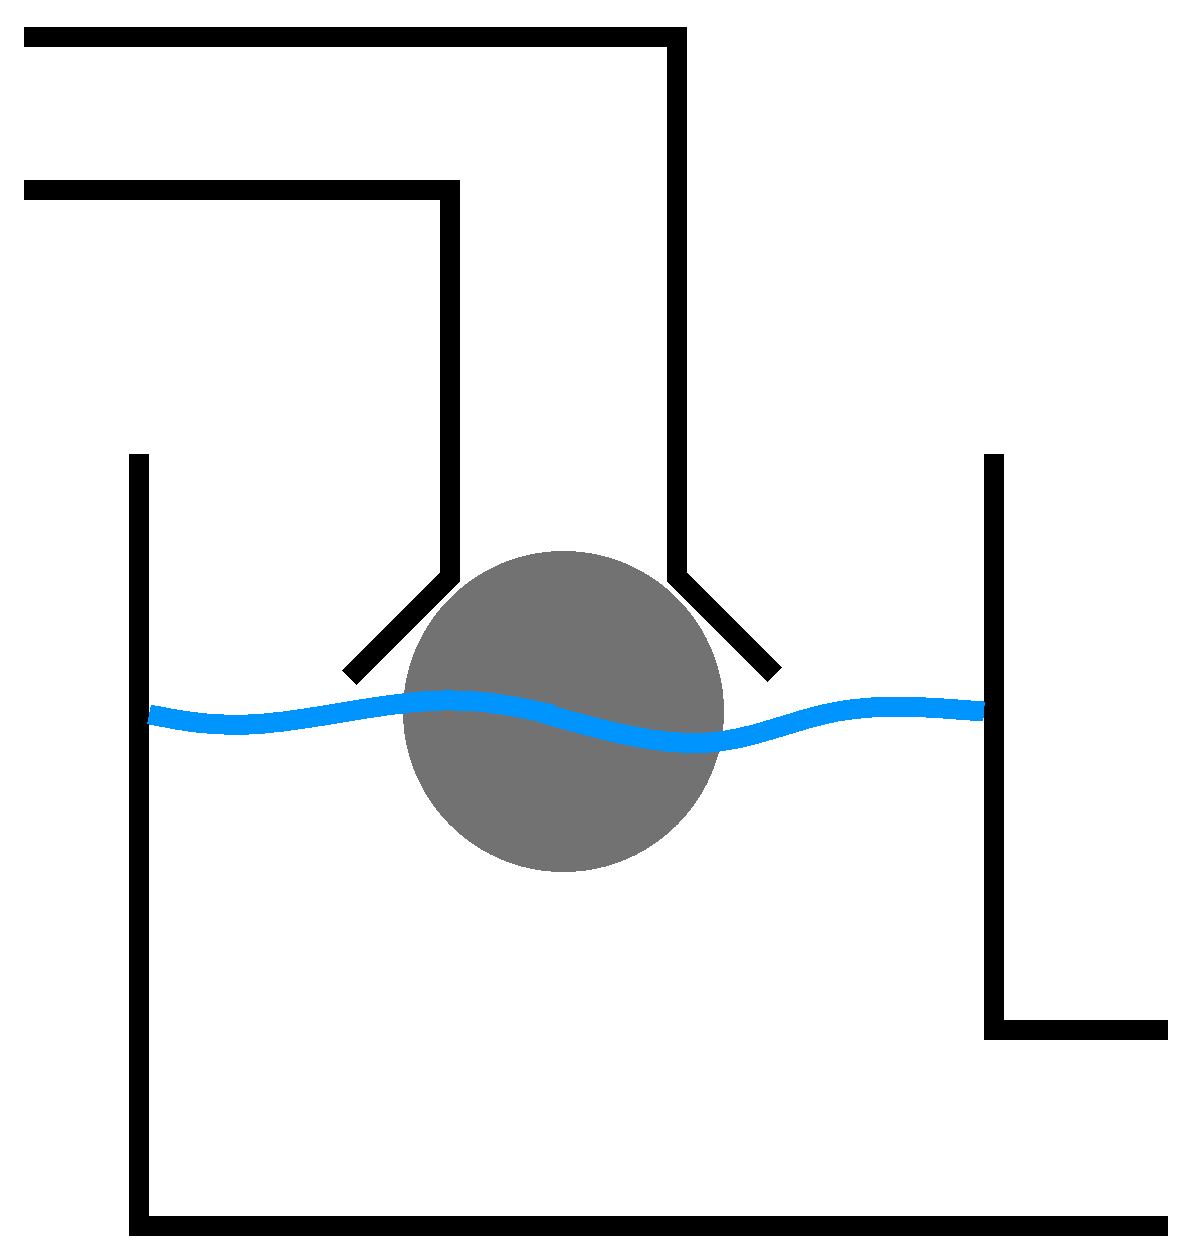
\includegraphics[scale=0.15]{images/ktesibius.png}
  \captionof{figure}{Zobrazowanie zasady działania regulatora Ktesibiosa}
  \label{fig:ktesibius}
\end{center}

Na przestrzeni kolejnych tysięcy lat w~technologii regulatorów nie dokonał się w~zasadzie żaden znaczący postęp. Dopiero w~XIX~i~XX~wieku rozpoczęły się badania nad teorią sterowania, w~których udział miało wielu naukowców z~całego świata. Lata prac doprowadziły do formalnego opracowania w~roku 1922 regulatora PID (ang.~\english{Proportional–Integral–Derivative}) (Definicja~\ref{def:pid}) przez rosyjskiego naukowca, Nicolasa Minorsky'ego\cite{bib:pidminorsky}.

\begin{Definition}[Regulator PID (Proporcjonalno-Integrująco-Różniczkujący)]\label{def:pid}
  Rrodzaj regulatora, który składa się z trzech elementów: proporcjonalnego (P), który reaguje na bieżącą wartość błędu (Definicja~ \ref{def:blad}) proporcjonalnie do niego; całkującego (I), który integruje bieżący błąd w czasie i reaguje na jego sumę; oraz różniczkującego (D), które reaguje na szybkość zmiany błędu. 
\end{Definition}

\begin{Definition}[Błąd; uchyb]\label{def:blad}
  W układach automatyki jest to różnica między wartością zadaną a zmierzoną wartością rzeczywistą.
\end{Definition}

Jego popularyzacja nastąpiła w~latach~'50~XX~wieku, gdy układy elektroniczne stały się tańsze, dotępniejsze i~bardziej niezawodne. Dziś jest powszechnie stosowany~w automatyce, robotyce, elektronice i~wielu innych dziedzinach inżynierii. Regulator PID jest stosowany najczęściej ze względu na prostotę, bardzo niski koszt implementacji i~wystarczające działanie w~większości przypadków.

Drugim najczęściej stosowanym regulatorem jest regulator predykcyjny MPC (ang.~\english{Model Predictive Control}). W~przeciwieństwie do tradycyjnych regulatorów które reagują na sprzężenie zwrotne z~wyjścia układu, regulator predykcyjny działa z~wyprzedzeniem, zanim zdąży nastąpić zmiana na wyjściu układu. 

Pierwsze wzmianki o~tym typie kontroli datowane są na wczesne lata '60~XX~wieku i~rozważania Rudolfa~E.~Kálmána na temat systemów liniowych. Od tego czasu, technologia regulatora predykcyjnego była rozwijana niezależnie przez wiele osób i~instytucji. W późnych latach '70~XX~wieku regulator ten można było już spotkać w ~zastosowaniach przemysłowych. W~roku 1979 zaprezentowano generację pierwszą, zaś najnowszą, 4~generację stanowią w~roku 1998\cite{bib:regulatormpc}. Pełna genealogia algorytmów MPC przedstawiona została na Rysunku~\ref{fig:regulatormpc}.

\begin{center}
  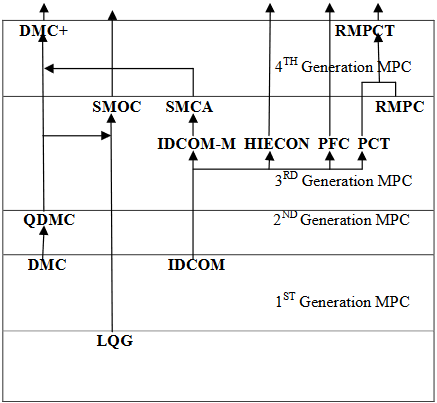
\includegraphics[scale=1]{images/drzewompc.png}
  \captionof{figure}{Genealogia algorytmów MPC\cite{bib:regulatormpc}}
  \label{fig:regulatormpc}
\end{center}

Regulatory predykcyjne znajdują zastosowanie w~układach o~dużym opóźnieniu i~wysokim rzędzie, gdzie regulatory PID są niewystarczające. Przykładem są sondy kosmiczne.

%%%%%%%%%%%%%% rozdział 3 - Wymagania i narzędzia %%%%%%%%%%%%%%%%%
\chapter{Założenia i narzędzia}
\label{ch:wymagania-i-narzedzia}

\begin{itemize}
\item wymagania funkcjonalne i niefunkcjonalne
\item przypadki użycia (diagramy UML) -- dla prac, w których mają zastosowanie
\item opis narzędzi, metod eksperymentalnych, metod modelowania itp.
\item metodyka pracy nad projektowaniem i implementacją -- dla prac, w których ma to zastosowanie
\end{itemize}

%%%%%%%%%%%%%% rozdział 4 - Projekt i wykonanie %%%%%%%%%%%%%%%%%
\chapter{Projekt i wykonanie}
\label{ch:04}

Jeśli „Specyfikacja zewnętrzna”:
\begin{itemize}
\item  wymagania sprzętowe i programowe
\item  sposób instalacji
\item  sposób aktywacji
\item  kategorie użytkowników
\item  sposób obsługi
\item  administracja systemem
\item  kwestie bezpieczeństwa
\item  przykład działania
\item  scenariusze korzystania z systemu (ilustrowane zrzutami z ekranu lub generowanymi dokumentami)
\end{itemize}

%%%%%%%%%%%%%%%%%%%%%
%% RYSUNEK Z PLIKU
%
%\begin{figure}
%\centering
%
\includegraphics[width=0.5\textwidth]{./politechnika_sl_logo_bw_pion_pl.pdf}
%\caption{Podpis rysunku zawsze pod rysunkiem.}
%\label{fig:etykieta-rysunku}
%\end{figure}
%Rys. \ref{fig:etykieta-rysunku} przestawia …
%%%%%%%%%%%%%%%%%%%%%
%
%%%%%%%%%%%%%%%%%%%%%
%% WIELE RYSUNKÓW 
%
%\begin{figure}
%\centering
%\begin{subfigure}{0.4\textwidth}
%    
\includegraphics[width=\textwidth]{./politechnika_sl_logo_bw_pion_pl.pdf}
%    \caption{Lewy górny rysunek.}
%    \label{fig:lewy-gorny}
%\end{subfigure}
%\hfill
%\begin{subfigure}{0.4\textwidth}
%    
\includegraphics[width=\textwidth]{./politechnika_sl_logo_bw_pion_pl.pdf}
%    \caption{Prawy górny rysunek.}
%    \label{fig:prawy-gorny}
%\end{subfigure}
%
%\begin{subfigure}{0.4\textwidth}
%    
\includegraphics[width=\textwidth]{./politechnika_sl_logo_bw_pion_pl.pdf}
%    \caption{Lewy dolny rysunek.}
%    \label{fig:lewy-dolny}
%\end{subfigure}
%\hfill
%\begin{subfigure}{0.4\textwidth}
%    
\includegraphics[width=\textwidth]{./politechnika_sl_logo_bw_pion_pl.pdf}
%    \caption{Prawy dolny rysunek.}
%    \label{fig:prawy-dolny}
%\end{subfigure}
%        
%\caption{Wspólny podpis kilku rysunków.}
%\label{fig:wiele-rysunkow}
%\end{figure}
%Rys. \ref{fig:wiele-rysunkow} przestawia wiele ważnych informacji, np. rys. \ref{fig:prawy-gorny} jest na prawo u góry.
%%%%%%%%%%%%%%%%%%%%%


 
\begin{figure}
\centering
\begin{tikzpicture}
\begin{axis}[
    y tick label style={
        /pgf/number format/.cd,
            fixed,   % po zakomentowaniu os rzednych jest indeksowana wykladniczo
            fixed zerofill, % 1.0 zamiast 1
            precision=1,
        /tikz/.cd
    },
    x tick label style={
        /pgf/number format/.cd,
            fixed,
            fixed zerofill,
            precision=2,
        /tikz/.cd
    }
]
\addplot [domain=0.0:0.1] {rnd};
\end{axis} 
\end{tikzpicture}
\caption{Podpis rysunku po rysunkiem.}
\label{fig:2}
\end{figure}

%%%%%%%%%%%%%% rozdział 5 - Eksperyment i weryfikacja %%%%%%%%%%%%%%%%%
\chapter{Eksperyment}
\label{ch:experiment}
Celem doświadczenia jest sprawdzenie, z~jaką dokładnością pojazd jest w~stanie docierać do wartości zadanej, innymi słowy jak bardzo zmniejszyć uchyb, utrzymując jednocześnie zsynchronizowane położenie silników. W tym celu zostaną podjęte następujące kroki:

\begin{enumerate}
    \item Doświadczalne wyznaczenie charakterystyki statycznej
    \item Strojenie równoległe regulatorów PID sygnałów niezależnych silnika prowadzącego i~śledzącego przy 50\%~prędkości i~1.5~m odległości
    \item Strojenie regulatora PID sygnału zależnego silnika śledzącego przy 50\%~prędkości i~1.5~m odległości
\end{enumerate}

Dodatkowym założeniem jest, że enkodery w~sposób idealny przekazują pulsy, a~sterownik i~licznik odbierają je również w sposób idealny i~żadnego nie gubią, ani nie są generowane dodatkowe poprzez szum elektryczny. W~ten sposób mając 2800 pulsów na obrót koła, dokładność pomiaru wynosi poniżej 1~mikrometra. Zakłada się więc że nie występuje błąd pomiarowy inny, niż ten spowodowany przez samo działanie pojazdu, takie jak dynamika wewnętrzna silników czy poślizg kół.

\section{Charakterystyka statyczna}
Została wyznaczona poprzez wysterowanie silników do stanu semi-ustalonego (ze względu na pewne drobne oscylacje), i~wyciągnięcie średniej z~15 pomiarów. Operację tę powtórzono dla obu silników, dla prędkości od 0\%~do 100\%,~ze skokiem~5\%. Wyznaczona została dla biegu jałowego. Można zauważyć, że dopiero gdzieś w~przedziale 5\%--10\% mocy, silniki pokonują opór statyczny i~zaczynają się obracać. Poza drobnymi odchyłkami wynikającymi z~niskiej jakości wykonania silników, oraz samej ich natury fizycznej, ich charakterystyki statyczne są w~przybliżeniu liniowe. Widać również, że nawet na biegu jałowym i~bez ograniczeń w~oprogramowaniu, prawy silnik jest o~kilka procent wolniejszy od lewego. Dokładnie to zjawisko, spowodowane m.in. drobnymi różnicami w~budowie fizycznej, postawiono za cel wyeliminować używając enkoderów i~regulatorów PID. Charakterystyka statyczna widoczna jest na Rysunku~\ref{fig:charstatjalowy}.


\begin{center}
    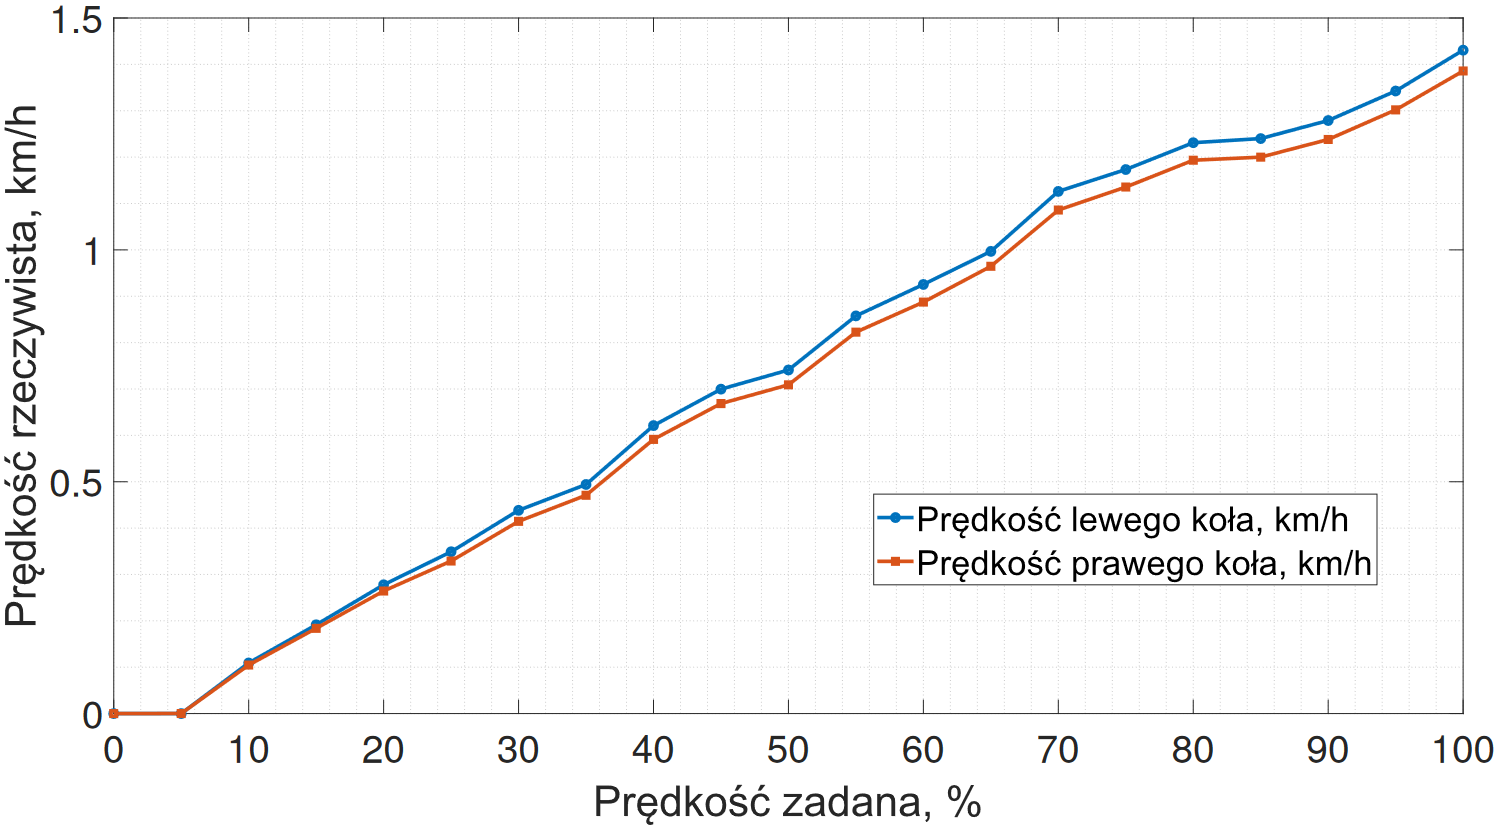
\includegraphics[scale=0.31]{images/charStat.png}
    \captionof{figure}{Charakterystyki statyczne silników}
    \label{fig:charstatjalowy}
\end{center}
\vspace*{-1cm}

\section{Strojenie regulatorów PID prowadzącego i śledzącego}
By ograniczyć ilość wykresów, których osobno byłoby kilkadziesiąt stron, kolejne iteracje zmiany tego samego parametru umieszczono na wspólnych wykresach. Strojenie odbywa się metodą doświadczalną.
\vspace*{-0.5cm}

\subsection*{Wzmocnienia proporcjonalne regulatora prowadzącego i~śledzącego}
Na Rysunku \ref{fig:strojeniekp} przedstawiono strojenie parametru K\textsubscript{P}.

\begin{center}
    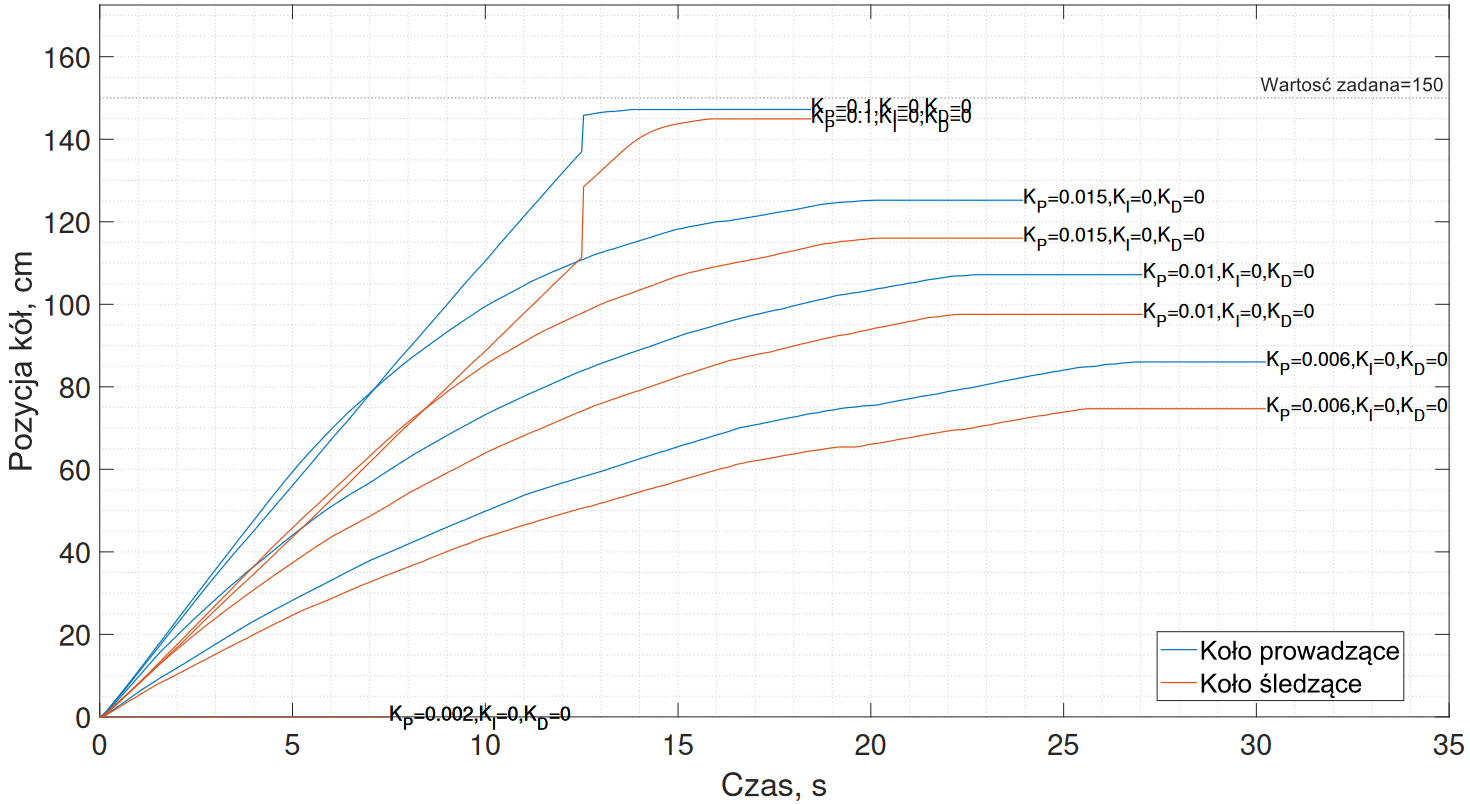
\includegraphics[scale=0.4]{images/strojenieKp.png}
    \captionof{figure}{Porównanie odpowiedzi układu na zmianę parametru K\textsubscript{P}}
    \label{fig:strojeniekp}
\end{center}

Widoczne jest, że wzmocnienie K\textsubscript{P}=0.002 jest zbyt małe, by pojazd ruszył z~miejsca (nie pokonuje oporu statycznego). Potrzebne jest wzmocnienie znajdujące się gdzieś w~przedziale K\textsubscript{P}$\in \left(0.002;0.006\right)$. Dla K\textsubscript{P}=0.1 uchyb jest bardzo mały, nawet bez części całkującej. Widoczny jest nagły skok odpowiedzi dla K\textsubscript{P}=0.1 pomiędzy 12~a~13~sekundą, którego powód jest nieznany. Jedną z~hipotez jest utracenie przez koła przyczepności na ułamek sekundy, tym samym wpadając w~lekki poślizg i~zwiększając obroty. Możliwy jest również inny błąd pomiaru.

\subsection*{Dodanie członu całkującego regulatora prowadzącego i śledzącego}
Na Rysunku \ref{fig:strojenieki} przedstawiono zmianę odpowiedzi układu po dodaniu parametru K\textsubscript{I} i~jednoczesnej modyfikacji K\textsubscript{P}.
\begin{center}
    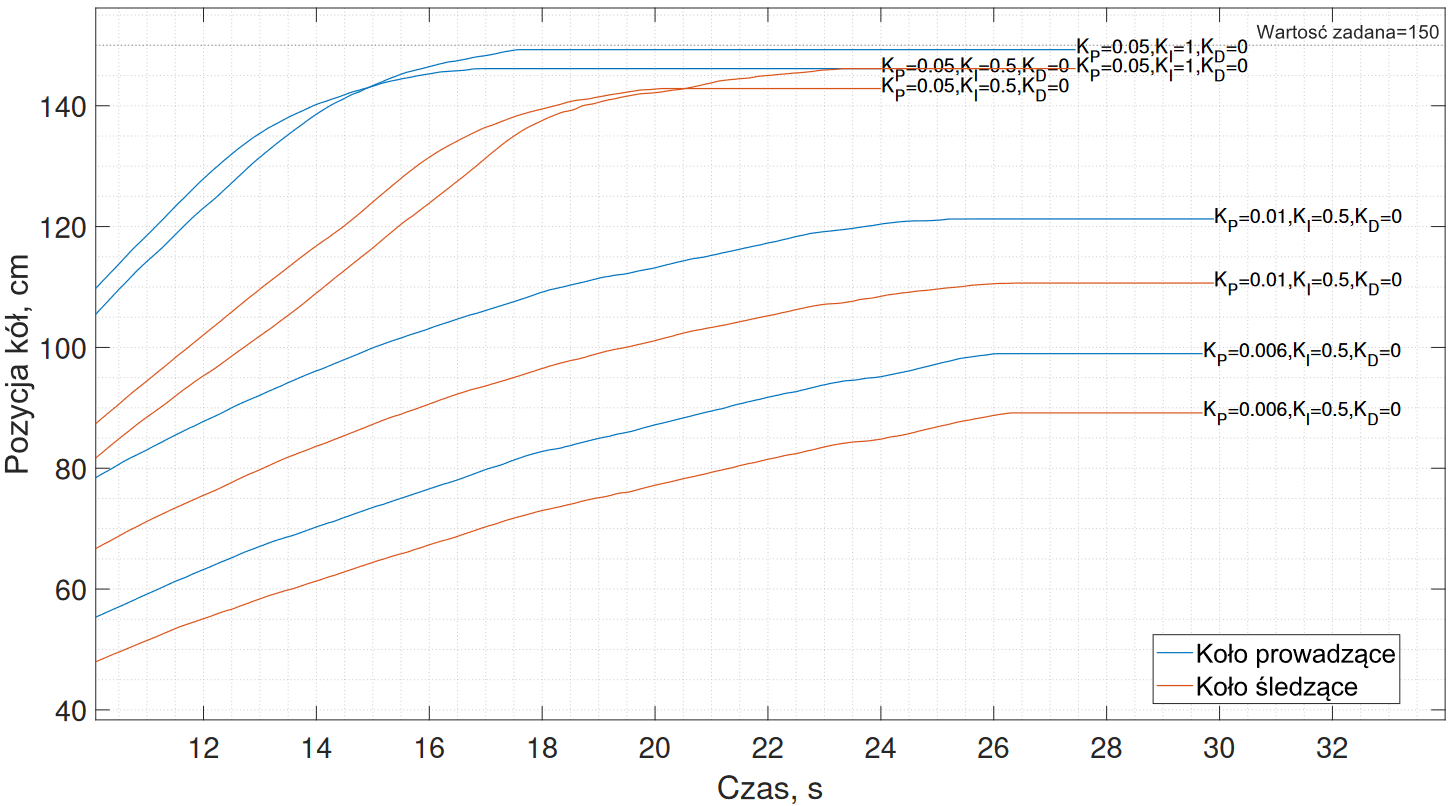
\includegraphics[scale=0.4]{images/strojenieKi.png}
    \captionof{figure}{Porównanie odpowiedzi układu na zmianę parametrów K\textsubscript{P} i K\textsubscript{I}}
    \label{fig:strojenieki}
\end{center}

Jak widać, nawet dla K\textsubscript{P}=0.05 czyli mniejszego niż najlepsze uzyskane w~poprzednim kroku, używając wzmocnienia K\textsubscript{I}=1, uchyb koła prowadzącego zostaje zniwelowany do wartości bliskiej 0. Jako że koło śledzące jest tym, które w~następnym kroku zostanie zsynchronizowane z~prowadzącym, a~samo koło prowadzące daje dobrą odpowiedź na aktualne parametry nie oscylując przy tym, wzmocnienie K\textsubscript{D} pozostanie wyzerowane, tym samym nie dodając do sygnału części różniczkującej regulatora.~W dalszych krokach używane będą parametry regulatorów K\textsubscript{P}=0.05, K\textsubscript{I}=1, oraz K\textsubscript{D}=0.

\section{Strojenie regulatora PID synchronizującego}
\subsection{Wzmocnienie różniczkujące}
Kolejnym krokiem jest dodanie regulatora PID synchronizującego koło śledzące z docelowym, zaczynając od części proporcjonalnej. Wykresy są zbyt blisko siebie by móc wyciągnąć wnioski, dlatego umieszczono dodatkowe przybliżenie. Różnice między poszczególnymi odpowiedziami w stanie ustalonym sprowadzają się do różnic w fizycznym wykonaniu przejazdu przez pojazd, czego należy się spodziewać. Strojenie wzmocnienia proporcjonalnego posiada mały wpływ na zbliżanie się do siebie odpowiedzi kół w części wykresu odpowiedzialnej za stan nieustalony. Odpowiedzi układu widoczne na Rysunku \ref{fig:strojenieskp}.

\begin{center}
    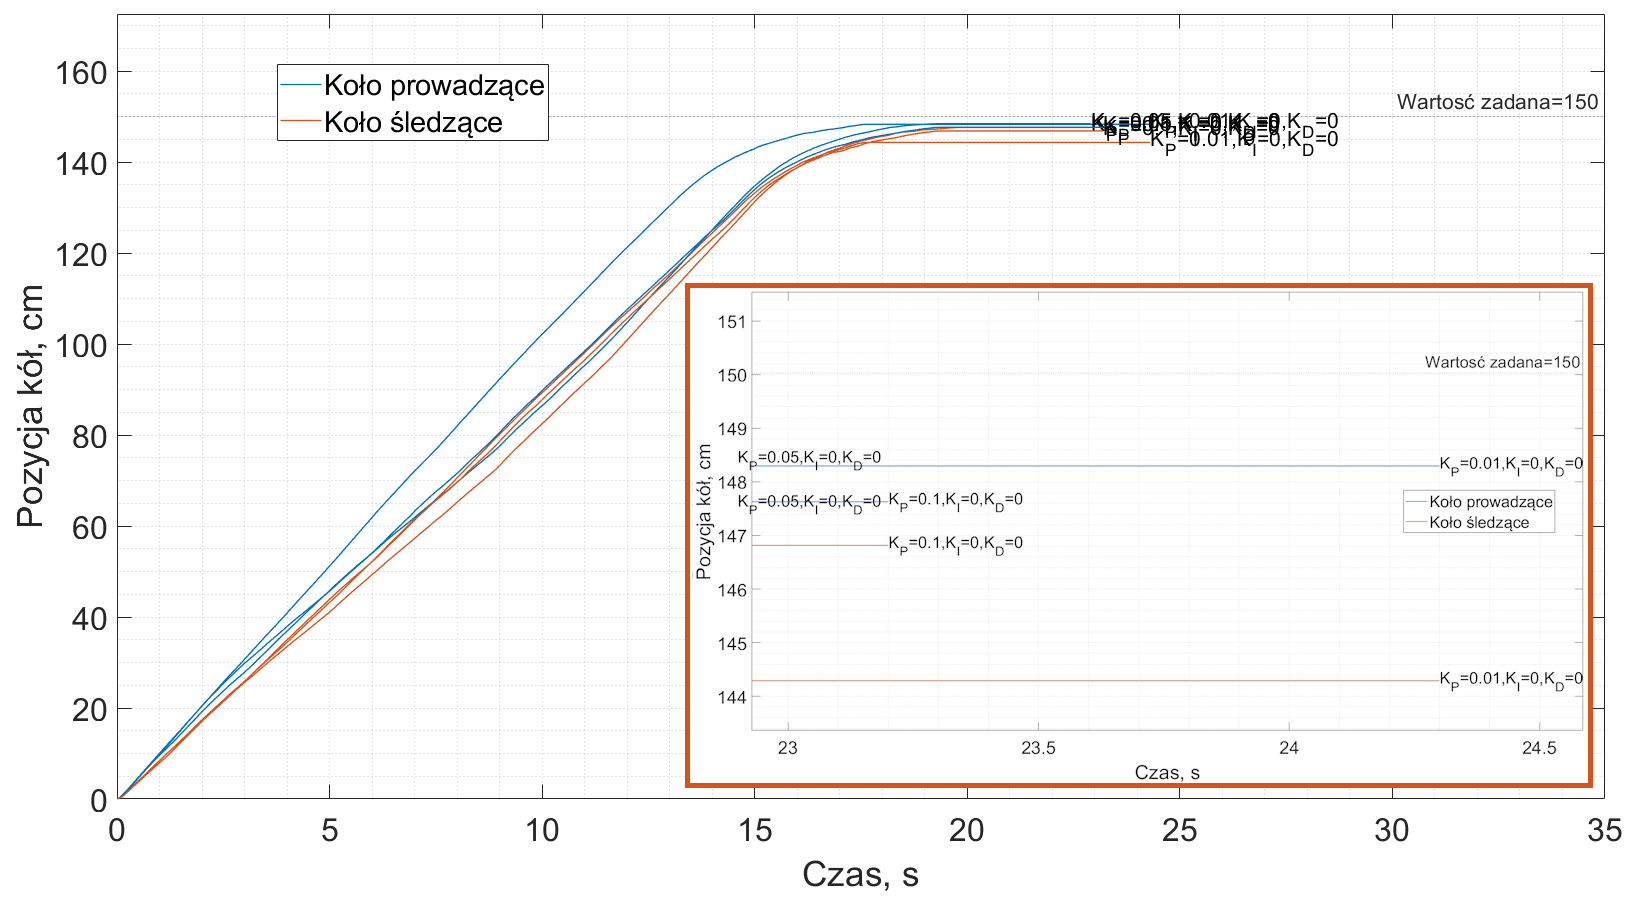
\includegraphics[scale=0.37]{images/strojenieSP.png}
    \captionof{figure}{Porównanie odpowiedzi układu na zmianę parametru K\textsubscript{P} regulatora synchronizującego}
    \label{fig:strojenieskp}
\end{center}

\subsection*{Dodanie składowej całkującej}
Po dodaniu członu całkującego do regulatora synchronizującego, zaczęły się widocznie wyłaniać pary kół z poszczególnych pomiarów. Wzmocnienie członu całkującego z powodzeniem zmniejszyło więc uchyb pomiędzy kołem prowadzącym a śledzącym, niestety nie do 0. Z wykresu ciężko odczytać konkretne pary i ich wartości, dlatego obliczenia przeprowadzono w MATLABie. Dla każdej próbki odjęto pozycję silnika śledzącego od prowadzącego. Następnie z otrzymanego wektora wyciągnięto średnią, a operację powtórzono dla wszystkich pomiarów (zmian K\textsubscript{I}), tym samym otrzymując wektor średnich błędów o długości równej ilości pomiarów. Najlepszym wynikiem charakteryzuje się K\textsubscript{I}=3, osiągając średni uchyb między pozycją kół na całym przebiegu na poziomie 0.12 cm. Przebiegi widoczne są na Rysunku \ref{fig:strojenieskpi}. Tak jak poprzednio, nie jest konieczne użycie członu różniczkującego.
\begin{center}
    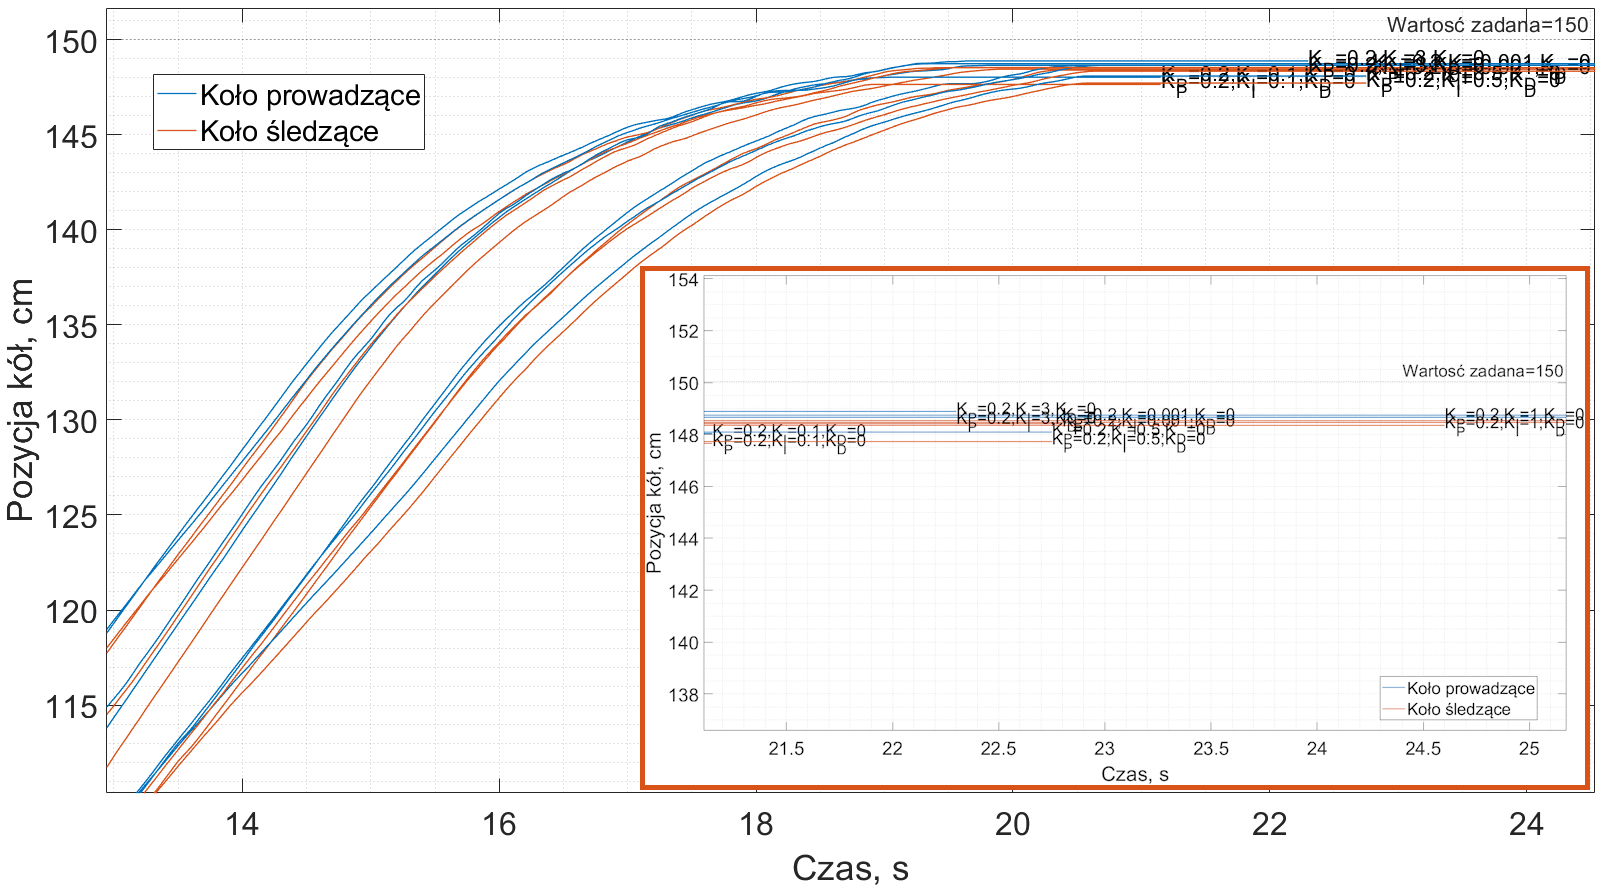
\includegraphics[scale=0.37]{images/strojenieSPI.png}
    \captionof{figure}{Porównanie odpowiedzi układu na zmianę parametru K\textsubscript{I} regulatora synchronizującego}
    \label{fig:strojenieskpi}
\end{center}

Dla najlepszego wyniku, na Rysunku \ref{fig:finalneprzebiegi} przedstawiono prędkość kół, oraz w Tabeli \ref{tab:finalneparametrypid} końcowe parametry PID.

\begin{center}
    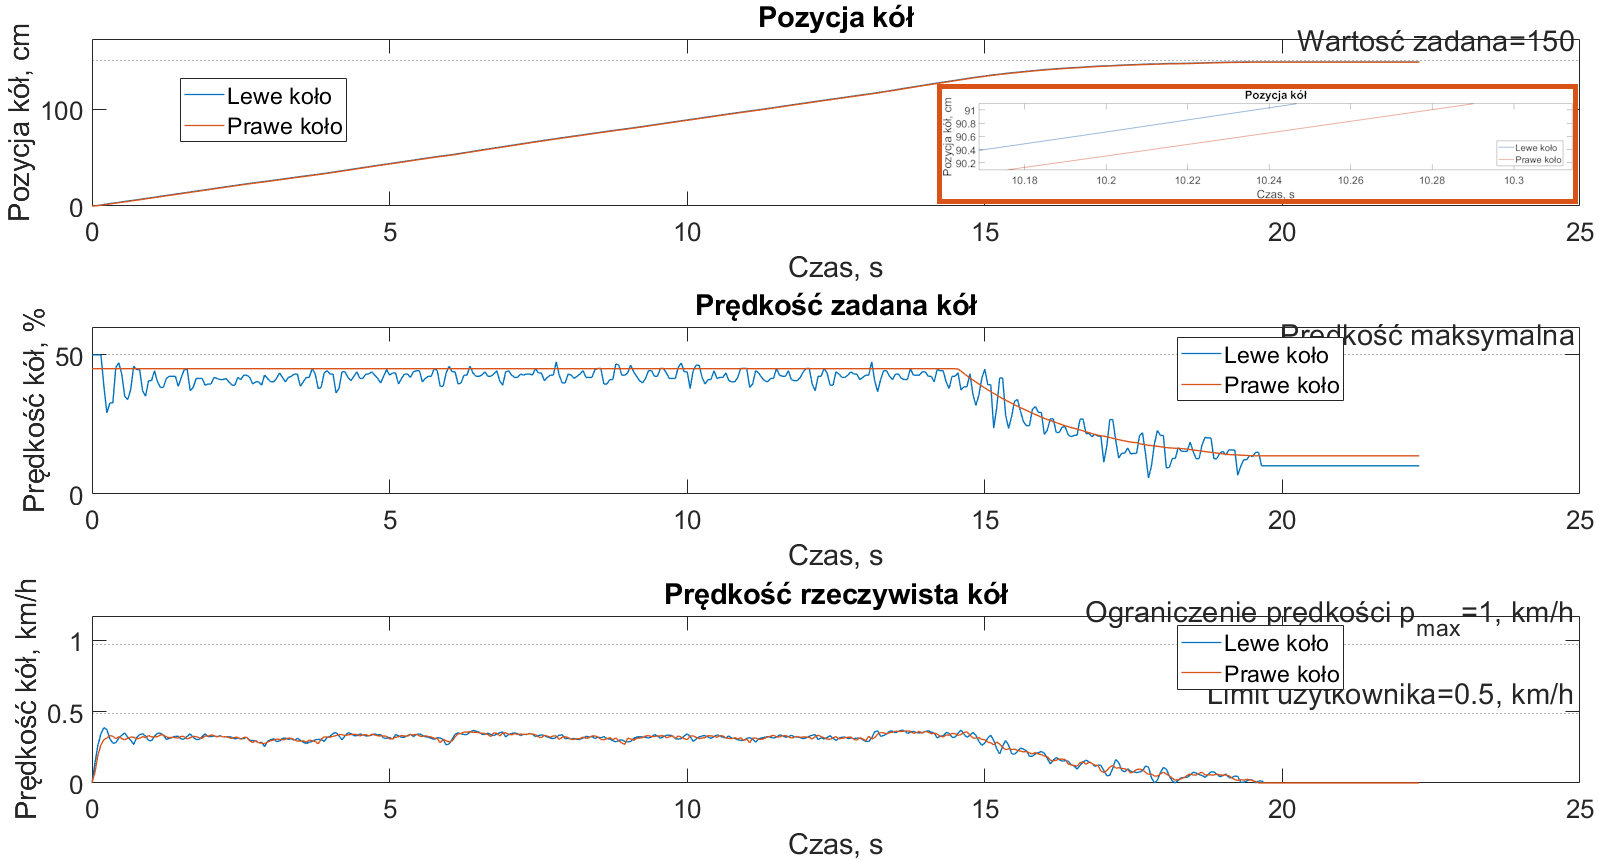
\includegraphics[scale=0.37]{images/wykresyfinalne.png}
    \captionof{figure}{Przedstawienie przebiegów pozycji silników oraz prędkości zadanej i rzeczywistej dla najlepszych parametrów PID}
    \label{fig:finalneprzebiegi}
\end{center}

\newpage

\begin{table}[!h]
\begin{tabular}{c|c|c|}
\cline{2-3}
\textbf{}                & Sygnały niezależne     & Sygnał zależny         \\ \hline
\multicolumn{1}{|c|}{K\textsubscript{P}} & 0.05                   & 0.2                    \\ \hline
\multicolumn{1}{|c|}{K\textsubscript{I}} & 1                      & 3                      \\ \hline
\multicolumn{1}{|c|}{K\textsubscript{D}} & \multicolumn{1}{c|}{0} & \multicolumn{1}{c|}{0} \\ \hline
\end{tabular}
\caption{Finalne parametry regulatorów PID dla najlepszego przebiegu}
\end{table}
\label{tab:finalneparametrypid}

Jak widać, dla finalnych parametrów uchyb od wartości zadanej jest bardzo mały, odczytany z wykresu wynosi 1.11 cm dla lewego koła i 1.46 cm dla prawego. Uchyb między kołami w stanie ustalonym wynosi --0.35 cm. Wyniki są więc bardzo dokładne biorąc pod uwagę warunki doświadczenia. Wadą są oscylacje prędkości zadanej lewego silnika spowodowane wysokim wzmocnieniem całkującym, które na szczęście w dużo mniejszym stopniu przekładają się na oscylacje realnej prędkości, oraz są zupełnie niewidoczne na przebiegu pozycji.

%%%%%%%%%%%%%% rozdział 6 - Podsumowanie i wnioski %%%%%%%%%%%%%%%%%
\chapter{Podsumowanie i wnioski}
Założenie początkowe dotyczące różnych rozmiarów kół - niespełnione.
Poprawić silnik na koło.
Nie zapomnij zmienić sekcji o matlabie (zwięszyła się ilość skryptów).


\backmatter
%\bibliographystyle{plplain}  % bibtex
%\bibliography{biblio} % bibtex
\printbibliography           % biblatex
\addcontentsline{toc}{chapter}{Bibliografia}

\begin{appendices}

%%%%%%%%%%%%%% rozdział 7 - Spis skrótów i symboli %%%%%%%%%%%%%%%%%
\chapter{Spis skrótów i symboli}
\begin{itemize}
\item[$u$] sygnał sterujący obiektem wykonawczym w układzie sterowania/regulacji
\item[PID] regulator Proporcjonalno-Całkująco-Różniczkujący (ang.~\english{Proportional–Integral–Derivative})
\item[MPC] regulator oparty na modelu predykcyjnym (ang.~\english{Model Predictive Control})
\item[DC] prąd stały (ang.~\english{Direct Current})
\item[LED] dioda emitująca światło (ang.~\english{Light Emitting Diode})
\item[3D] 3 wymiary (ang.~\english{3 dimensions})
\item[Wi-Fi] sieć bezprzewodowa (ang.~\english{Wireless Fidelity})
\item[RTOS] system czasu rzeczywistego (ang.~\english{Real Time Operating System})
\item[FDM] modelowanie przez nakładanie stopionego materiału (ang.~\english{Fused Deposition Modeling})
\item[DLP] modelowanie przez utwardzanie materiału światłem (ang.~\english{Digital Light Processing})
\item[PLA] polilaktyd (ang.~\english{Polylactic Acid})
\item[LIDAR] detekcja światła i pomiar odległości (ang.~\english{LIDAR})
\end{itemize}

%%%%%%%%%%%%%% rozdział 8 - Źródła %%%%%%%%%%%%%%%%%
\chapter{Źródła}
\vspace*{-0.5cm} % poprawia pojedynczą linijkę na następnej stronie
% łączność, pętla while(true)
\lstinputlisting[language=c++, label={lst:conwhiletrue}, firstline=141, lastline=151, firstnumber=141, caption={Connectivity.cpp, pętla \english{while(true)} zadania podtrzymującego połączenie Wi-Fi}]{code/Connectivity.cpp}

% klient UDP, pętla while(true)
\lstinputlisting[language=c++, label={lst:udpclientwhiletrue}, firstline=214, lastline=224, firstnumber=214, caption={Connectivity.cpp, pętla \english{while(true)} zadania klienta UDP}]{code/Connectivity.cpp}

% pętla regulatora
\lstinputlisting[language=c++, label={lst:petlaregulatora}, firstline=90, lastline=132, firstnumber=90, caption={Controller.cpp, funkcja wywoływana przez zegar cykliczny}]{code/Controller.cpp}

% regulator
\lstinputlisting[language=c++, label={lst:regulator}, firstline=70, lastline=88, firstnumber=70, caption={Controller.cpp, funkcja regulatora wywoływana wewnątrz funkcji wywoływanej przez zegar cykliczny}]{code/Controller.cpp}

%%%%%%%%%%%%%% rozdział 9 - Lista dodatkowych plików, uzupełniających tekst pracy %%%%%%%%%%%%%%%%%
\chapter{Lista dodatkowych plików, uzupełniających tekst pracy} 
Work in progress.

\listoffigures
\addcontentsline{toc}{chapter}{Spis rysunków}
\listoftables
\addcontentsline{toc}{chapter}{Spis tabel}

\end{appendices}
\end{document}


%% Finis coronat opus.